\section{Introduction}
\label{sec:introduction}

% state the learning objective 
The purpose of this laboratory assignment is to make a Bandpass filter using OP-AMP, with the goal to get the highest merit, M, possible.
$$ M = \frac{1}{cost \times gainDeviation \times centralFreqDev}$$

Using the simplified circuit shown in Figure~\ref{fig:t5}, we tested different values for the resistors and capacitors and we found that the values in Table~\ref{tab:values} yielded the best merit. However, to get to those values, the real circuit in Figure~\ref{fig:t5-real} was used.

In Section~\ref{sec:simulation}, the circuit is analyzed by simulation using the software Ngspice. 

In Section~\ref{sec:analysis}, the circuit is analyzed theoretically using the software GNU Octave. 

In Section~\ref{sec:comparison}, a comparison is done between the results obtained by both analyses, theoretical and simulation, and a practical .

The conclusions of this study are outlined in Section~\ref{sec:conclusion}.

\begin{table}[ht!]
    \centering
    \begin{tabular}{c c}
    \toprule
    Component & Value \\ \midrule
    $C_1$  & 220 $nF$      \\
    $C_2$  & 110 $nF$      \\
    $R_1$  & 1 $k\Omega$   \\
    $R_2$  & 1 $k\Omega$   \\
    $R_3$  & 150 $k\Omega$ \\
    $R_4$  & 1 $k\Omega$   \\ \bottomrule
    \end{tabular}
    \caption{Resistance and Capacitance for the components}
    \label{tab:values}
\end{table}

\begin{figure}[ht!]
\centering
    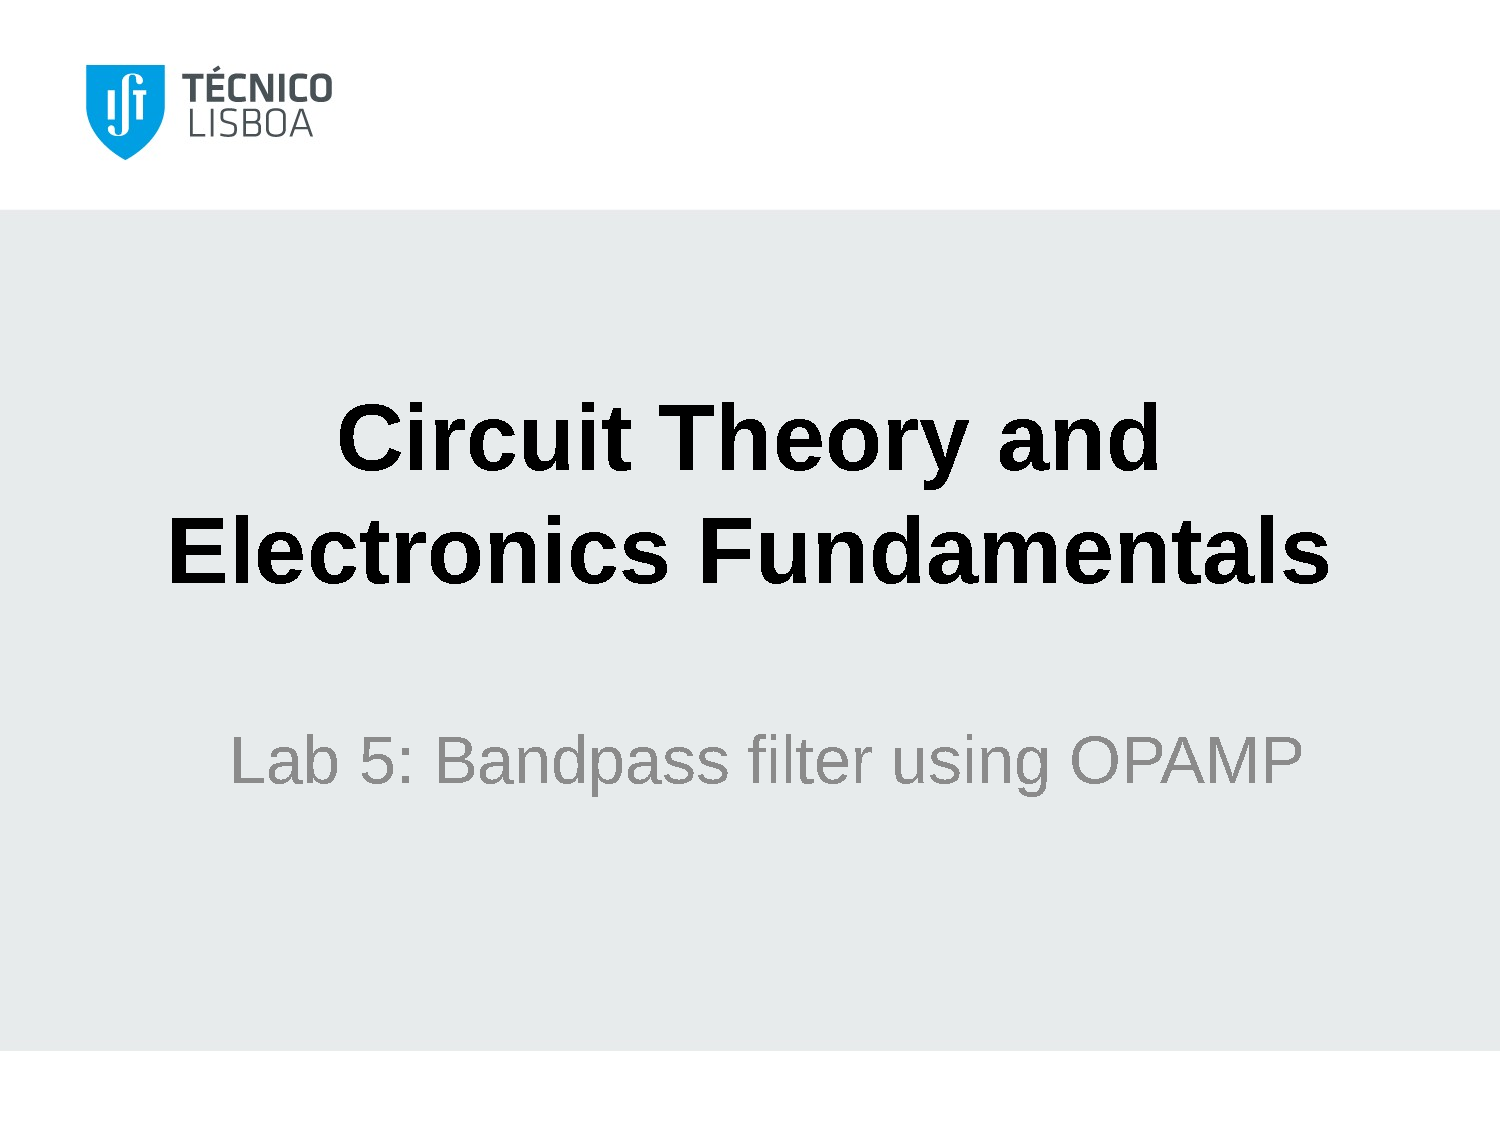
\includegraphics[width=0.8\linewidth]{t5.pdf}
\caption{Circuit T5, simplified.}
\label{fig:t5}
\end{figure}

\begin{figure}[ht!]
\centering
    \includegraphics[width=0.8\linewidth]{t5-real.pdf}
\caption{Circuit T5, real.}
\label{fig:t5-real}
\end{figure}

\FloatBarrier
\clearpage
